\documentclass[10pt,a4paper,oneside]{book}

\usepackage[left=2.5cm,right=2.5cm,top=2.5cm,bottom=3cm]{geometry}
\usepackage[utf8]{inputenc}
\usepackage{palatino}
\usepackage[T1]{fontenc}
\usepackage{graphicx}
\graphicspath{{../images/}}
\usepackage{hyperref}
\urlstyle{same}
\usepackage{amsmath}
\usepackage{amsfonts}
\usepackage{amssymb}
\usepackage{circuitikz}

\begin{document}
\setlength{\parindent}{0pt}
\setlength{\parskip}{6pt}

% Title page
 \vspace*{3cm}
	
 \begin{center}
 	\Huge eistoolbox \par
 \end{center}
 \begin{center}
 	\LARGE for \par
 \end{center}
 \begin{center}
 	\Huge MathWorks\textsuperscript{\textregistered} MATLAB \par
 \end{center}
 
 \vspace*{2cm}
 
\begin{center}
	\Large A toolbox for batch fitting of Electrochemical Impedance Spectroscopy data to equivalent circuit models
\end{center} 
 
 \vspace*{2cm}
 
 \begin{center}
 	\Huge User Guide \par
 \end{center}
 \begin{center}
 	\LARGE Juan J. Montero-Rodríguez \par
 \end{center}
 
 \vspace*{4cm}
 
 \begin{center}
 	\Large Version 0.1-54
 \end{center}

\clearpage

\tableofcontents

\chapter{Introduction}

\textbf{eistoolbox} is a toolbox for MATLAB\textregistered{} used for batch fitting Electrochemical Impedance Spectroscopy (EIS) data to equivalent circuits. 

Currently it is \textbf{alpha software}, and it will evolve over time.

\section{Impedance Spectroscopy}

Electrochemical Impedance Spectroscopy (EIS) measures the complex impedance of a sample as a function of the frequency. The experimental results are stored in two possible formats: polar coordinates (magnitude and phase) or rectangular coordinates (real and imaginary).

\begin{align} \label{impedance}
	Z(f) = R + jX
\end{align}

where R is the resistance and X is the reactance of the sample.

The real part of the impedance is proportional to the resistivity, and the imaginary part is proportional to the permittivity. Both parameters can be calculated directly from the measurements, considering the exact geometry of the electrodes and measurement setup. For parallel plate electrodes, the following equations apply:

\begin{align}
R = \dfrac{\rho L}{A} \label{resistance} \\
C = \dfrac{\epsilon A}{D} \label{capacitance}
\end{align}

The capacitive reactance is given by

\begin{align}
X_C = \dfrac{1}{2\pi{}fC}	\label{reactivecapacitance}
\end{align}

Substituting \eqref{capacitance} and \eqref{reactivecapacitance} into \eqref{impedance} results in the following equation, which describes the impedance in terms of the resistivity and permittivity of the sample between parallel electrodes:

\begin{align}
Z(f) = \dfrac{\rho L}{A} + \dfrac{1}{2\pi{}f} \dfrac{D}{\epsilon A}
\end{align}

Impedance Spectroscopy is also referred as Dielectric Spectroscopy, because it gives information about the dielectric properties of the measured sample.



\clearpage
\section{Equivalent Circuits}

Experimental data is fitted to equivalent circuit models. The models are designed to describe the interfaces, chemical processes and boundaries of the measured setup.

\subsection{Circuit Elements}

The elements present in the software are described in Table \ref{circelements}:

\begin{table}[h]
	\centering
	\caption{Equivalent circuit elements and their MATLAB implementation.}
	\label{circelements}
	\begin{tabular}{llll}
		\hline \textbf{Symbol} & \textbf{Element} & \textbf{Equation} & \textbf{MATLAB expression}\\
		\hline R1 & Resistor & $Z(f) = R$ & \verb|z=p*ones(size(f))| \\ 
		C1 & Capacitor & $Z(f) = 1 / j 2\pi fC$ & \verb|z=1./(1i*2*pi*f*p)| \\ 
		L1 & Inductor & $Z(f) = j 2\pi fL$  & \verb|z=1i*2*pi*f*p| \\
		E2 & Constant Phase Element & $Z(f) = 1 / p_1 (j 2 \pi f)^{p_2} $ & \verb|z=1./(p(1)*(1i*2*pi*f).^p(2))| \\
		\hline
	\end{tabular}
\end{table}

The Warburg element can be obtained with a Constant-Phase Element by setting $p_2=0.5$


\subsection{Circuit String Syntax}

Circuits can be built using series and parallel combinations of the elements in Table \ref{circelements}, using the series and parallel operators s() and p(). These operators can contain any number of elements, separated by commas.

The number next to the element letter is the number of free parameters for this element. For a capacitor (C1) the only free parameter is the capacitance. For the constant-phase element (E2) the free parameters are p1 and p2.

\textbf{Common mistake:} Do not write the circuit elements as s(R1,R2,R3,C4...). The elements cannot be written as labels. Instead, write s(R1,R1,R1,C1...).

\subsection{Circuit Files (.ckt)}

The circuit string, initial parameters and boundary conditions can be stored and loaded from a circuit file with the .ckt extension. This file is read by MATLAB line-to-line.

Check the folder 'examples\_circuits' for more examples.

\begin{center}
\fbox{ \parbox{14cm}{
	\textbf{Example 1: Voigt model in the form R+R//C+R//C+R//C}
		
	\begin{circuitikz}
		\draw 
		(0,0) to[R=$R_S$] (2,0)
		(2,0) to[short] (2,2)
		(2,2) to[C=$C_1$] (4,2) % The resistor
		(4,2) to[short] (4,0)
		(2,0) to[R=$R_1$] (4,0)
		(4,0) to[R=$R_2$] (6,0)
		(6,0) to[R=$R_3$] (8,0)
		(4,2) to[C=$C_2$] (6,2)
		(6,2) to[short] (6,0)
		(6,2) to[C=$C_3$](8,2)
		(8,2) to[short] (8,0)
		(8,0) to[short] (10,0);
	\end{circuitikz}
	
	\textbf{Recommended circuit file:}
	
	s(R1,p(R1,C1),p(R1,C1),p(R1,C1))	\% circuit string
	
	[100,100,1e-6,100,1e-6,100,1e-6]	\% initial parameters
	
	[0,0,0,0,0,0,0]						\% lower boundary conditions
	
	[inf,inf,inf,inf,inf,inf,inf]		 \% upper boundary conditions
	
	}
}
\end{center}

\begin{center}
	\fbox{ \parbox{14cm}{
			\textbf{Example 2: Ladder circuit in the form: ((((R//C)+R)//C)+R)//C+R}
			
			\begin{circuitikz}
				\draw 
				(6,0) to[R=R3] (8,0)
				(8,0) to[short] (8,2)
				(6,0) to[short] (6,2)
				(6,2) to[C=C3] (8,2)
				(4,2) to[R=R2] (6,2)
				(4,2) to[short] (4,4)
				(4,4) to[C=C2] (6,4)
				(6,4) to[short] (8,4)
				(2,4) to[R=R1] (4,4)
				(2,4) to[short] (2,6)
				(2,6) to[C=C1] (4,6)
				(4,6) to[short] (8,6)
				(0,6) to[R=RS] (2,6)
				(8,6) to[short] (8,0)
				(8,6) to[short] (10,6)
				;
			\end{circuitikz}
			
			\textbf{Recommended circuit file:}
			
			s(p(s(p(s(p(R1,C1),R1),C1),R1),C1),R1)	\% circuit string
			
			[100,1e-6,100,1e-6,100,1e-6,100]	\% initial parameters... order: R3,C3,R2,C2,R1,C1,RS
			
			[0,0,0,0,0,0,0]						\% lower boundary conditions
			
			[inf,inf,inf,inf,inf,inf,inf]		 \% upper boundary conditions
			
		}
	}
\end{center}



\chapter{Current capabilities of this software}

It can accept any number of input files, both in CSV and Gamry DTA formats.

The CSV files should contain three columns with the impedance data, in the order: FREQ,REAL,IMAG. 

The imaginary part can be positive or negative; the absolute value is taken inside the program before plotting.

The fitting algorithm uses the "fminsearch" function, implemented using the Zfit library from Jean-Luc Dellis. 

It accepts any type of circuit model, built with serial and parallel elements, in the Zfit circuit string format.

The currently implemented elements are: resistors, capacitors, inductors and constant-phase elements (CPE). 

The Warburg element can be implemented by using a CPE and setting the second parameter to 1/2.


\section{Planned updates}

In the future it will accept Levenberg-Marquard, Nelder-Mead, BFGS and Powell algorithms.

It will also include the error percentages of every fitting parameter, as well as the Pearson coefficient and correlation plot of the fitting results.


\chapter{Using the eistoolbox}

\section{Quick start guide}

1. Add files using the "Add file..." button

2. Write the circuit string and fitting parameters (circuit string formatting)

3. Click the "Fit" button

4. Save the results using the "Save..." button

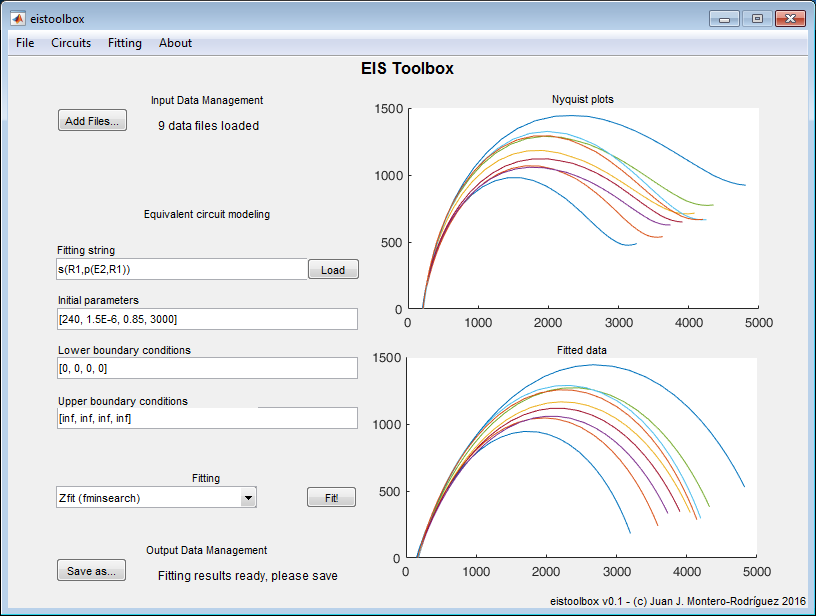
\includegraphics[width=15cm]{main_screenshot.png}

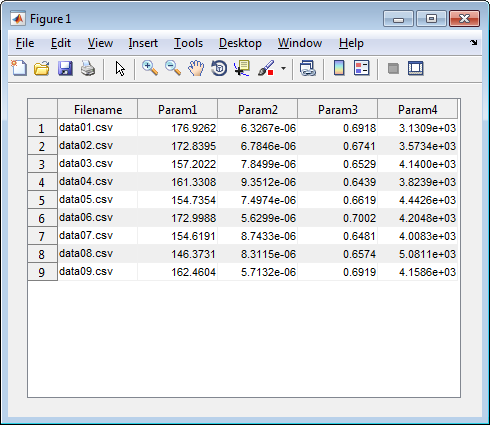
\includegraphics[width=10cm]{scr_results.png}


\chapter{Fitting Algorithms}

The fitting algorithms of this toolbox reduce the following distance function:


\begin{verbatim}
function dist=distance(param)
    ymod=feval(handlecomputecircuit,param,circuitstring,freq);
    if isequal('fitNP',fitstring)
        dist=sum(sum((ymod-zrzi).^2));
    else
        dist=sum(sum(((ymod-zrzi)./zrzi).^2));  
    end
end
\end{verbatim}


For \textbf{non-proportional fitting} the algorithm minimizes the squared difference between fitted (observed) and measured (expected) data.

\[ d = \sum(o-e)^2 \]

For \textbf{proportional fitting} the algorithm calculates the squared difference between fitted (observed) and measured (expected) data, divided by the measured (expected) data, in a way similar to the Pearson's chi-square test:

\[ d = \chi^2 = \sum \dfrac{(o-e)^2}{e} \]

If the experimental impedance curve matches exactly the simulated curve, the distance function would have a value of zero.

To minimize the distance function, the toolbox adjusts the input parameters and recalculates the simulated data in each iteration. This is done in the second line of the code from above.

\section{fminsearchbnd}

This function was written by John D'Errico and published on MathWorks MATLAB Central under an open-source license. The original file can be downloaded at \url{https://de.mathworks.com/matlabcentral/fileexchange/8277-fminsearchbnd--fminsearchcon}.

The function is based on fminsearch and includes the possibility of using boundary conditions, such as the lower and upper limits for the individual circuit parameters.

\section{Other algorithms}

The following optimization algorithms are not yet implemented in this toolbox. These are some of the most used algorithms for fitting EIS data to equivalent circuit models.

\begin{itemize}
	\item Levenberg-Marquardt
	\item Nelder-Mead
	\item BFGS
	\item Powell
\end{itemize}



\chapter{Statistics}

The program computes the following statistical parameters:

\section{Linear regressions}

Real of fitted vs Real of measured

Imag of fitted vs Imag of measured

MAG of fitted vs MAG of measured

\section{Chi-square goodness of fit}

\[ \chi^2 = \sum_i^n{\dfrac{(Observed_i-Expected_i)^2}{Expected_i}} \]

Observed= fitted data

Expected= measured data

\section{Error estimates for individual parameters}

ToDo


\newpage{}
\chapter{Licenses for included software}

\section{Zfit}

The original file was released in 2005 and it is available here:\\

\url{https://de.mathworks.com/matlabcentral/fileexchange/19460-zfit}

\begin{small}
\begin{verbatim}
Copyright (c) 2005, Jean-Luc Dellis
All rights reserved.

Redistribution and use in source and binary forms, with or without
modification, are permitted provided that the following conditions are
met:

* Redistributions of source code must retain the above copyright
notice, this list of conditions and the following disclaimer.
* Redistributions in binary form must reproduce the above copyright
notice, this list of conditions and the following disclaimer in
the documentation and/or other materials provided with the distribution

THIS SOFTWARE IS PROVIDED BY THE COPYRIGHT HOLDERS AND CONTRIBUTORS "AS IS"
AND ANY EXPRESS OR IMPLIED WARRANTIES, INCLUDING, BUT NOT LIMITED TO, THE
IMPLIED WARRANTIES OF MERCHANTABILITY AND FITNESS FOR A PARTICULAR PURPOSE
ARE DISCLAIMED. IN NO EVENT SHALL THE COPYRIGHT OWNER OR CONTRIBUTORS BE
LIABLE FOR ANY DIRECT, INDIRECT, INCIDENTAL, SPECIAL, EXEMPLARY, OR
CONSEQUENTIAL DAMAGES (INCLUDING, BUT NOT LIMITED TO, PROCUREMENT OF
SUBSTITUTE GOODS OR SERVICES; LOSS OF USE, DATA, OR PROFITS; OR BUSINESS
INTERRUPTION) HOWEVER CAUSED AND ON ANY THEORY OF LIABILITY, WHETHER IN
CONTRACT, STRICT LIABILITY, OR TORT (INCLUDING NEGLIGENCE OR OTHERWISE)
ARISING IN ANY WAY OUT OF THE USE OF THIS SOFTWARE, EVEN IF ADVISED OF THE
POSSIBILITY OF SUCH DAMAGE.
\end{verbatim}
\end{small}


\end{document}
